\documentclass[letterpaper,twocolumn,openany]{dndbook}

% Use babel or polyglossia to automatically redefine macros for terms
% Armor Class, Level, etc...
% Default output is in English; captions are located in lib/dndstring-captions.sty.
% If no captions exist for a language, English will be used.
%1. To load a language with babel:
%	\usepackage[<lang>]{babel}
%2. To load a language with polyglossia:
%	\usepackage{polyglossia}
%	\setdefaultlanguage{<lang>}
\usepackage[english]{babel}
%\usepackage[italian]{babel}
% For further options (multilanguage documents, hypenations, language environments...)
% please refer to babel/polyglossia's documentation.

\usepackage[utf8]{inputenc}
\usepackage[singlelinecheck=false]{caption}
\usepackage{lipsum}
\usepackage{listings}
\usepackage{shortvrb}
\usepackage{stfloats}

\captionsetup[table]{labelformat=empty,font={sf,sc,bf,},skip=0pt}

\MakeShortVerb{|}

\lstset{
    basicstyle=\ttfamily,
    language=[LaTeX]{TeX},
}

\ExplSyntaxOn
%%%%%%%%%%%%%%%%%%%%%%%%%%%%%%%%%%%%%%%%%%%%%%%%%%%%%%%%%%%%%%%%%%%%%%%%%%%%%%
% Special command for psionic manifestations.
%%%%%%%%%%%%%%%%%%%%%%%%%%%%%%%%%%%%%%%%%%%%%%%%%%%%%%%%%%%%%%%%%%%%%%%%%%%%%%
% #1 - Name
% #2 - Level and school
% #3 - Casting time
% #4 - Range
% #5 - Charges
% #6 - Duration
\NewDocumentCommand {\DndPsiHeader} { m m m m m m }
  {
    \DndItemHeader {#1} {#2}

    \begin{description}
      [
        nosep,
        labelsep = \l__dnd_space_dim,
        after    = { \vspace{4pt plus 1pt minus 1pt} },
      ]
      \item [ \spellcastingtimename : ] #3
      \item [ \spellrangename       : ] #4
      \item [ Charges: ] #5
      \item [ \spelldurationname    : ] #6
    \end{description}
  }
\ExplSyntaxOff

% Start document
\begin{document}
\footnotesize

\chapter{Psionics}
The gemstone dragons are silico-organic organisms. When hatched, they are almost entirely organic. As they grow, their crystalline structure grows, as does their psionic power.\\
The crystals that grow on and thread through their bodies form a network of psionic filaments that capture, conduct, amplify, and store charges of psionic energies, which the dragons then convert into \textbf{manifestations}.\\
% Each dragon begins with a number of charges based on their age. They can expend these charges to cast any psionic manifestation. Many of these manifestations have a base cost and can be enhanced by expending more charges.\\
% Over time, the dragon’s crystals conduct more psionic energies into its body, recharging its power. \textbf{At the end of each of its turns, roll the recharge die and restore that many charges.}\\
% Each dragon also has a \textbf{Fracture score}. Each time it takes more damage than its Fracture score in a single turn, its crystalline form fractures, diminishing its ability to recharge its power. Roll the recharge die and reduce the dragon’s maximum charges by the result. This damage heals itself upon finishing a long rest.

\section{Items}

\DndItemHeader{Psionic Crystal}{Wondrous item, rare, requires attunement}
Chipped off the hide of a gemstone dragon, this crystal grants you psionic abilities depending on its size. It recharges upon completing a long rest. If you ever use the last charge, it turns into an inert precious stone.

\begingroup
\DndSetThemeColor[PhbMauve]

\begin{table*}[b]
    \begin{DndTable}[width=\linewidth,header=Crystal Powers by Size]{lllllX}
        \textbf{Size} & \textbf{Example} & \textbf{Charges} & \textbf{Recharge} & \textbf{Save DC} & \textbf{Manifestations} \\
        Small & a coin & 8 & 1d4 & DC 13 & Amplify, Distance, Flay, Psionic Spell \\
        Medium & an apple & 12 & 1d6 & DC 14 & Amplify, Distance, Flay, Forget, Psionic Spell, Sympathy \\
        Large & a bowl & 16 & 1d8 & DC 15 & Amplify, Distance, Flay, Forget, Mindscape, Psionic Spell, Reflection, Sympathy \\
        Huge & a pumpkin & 24 & 1d10 & DC 16 & Amplify, Distance, Elsewhere, Flay, Forget, Mindscape, Psionic Spell, Reflection, Sympathy
    \end{DndTable}
\end{table*}

\begin{figure}
    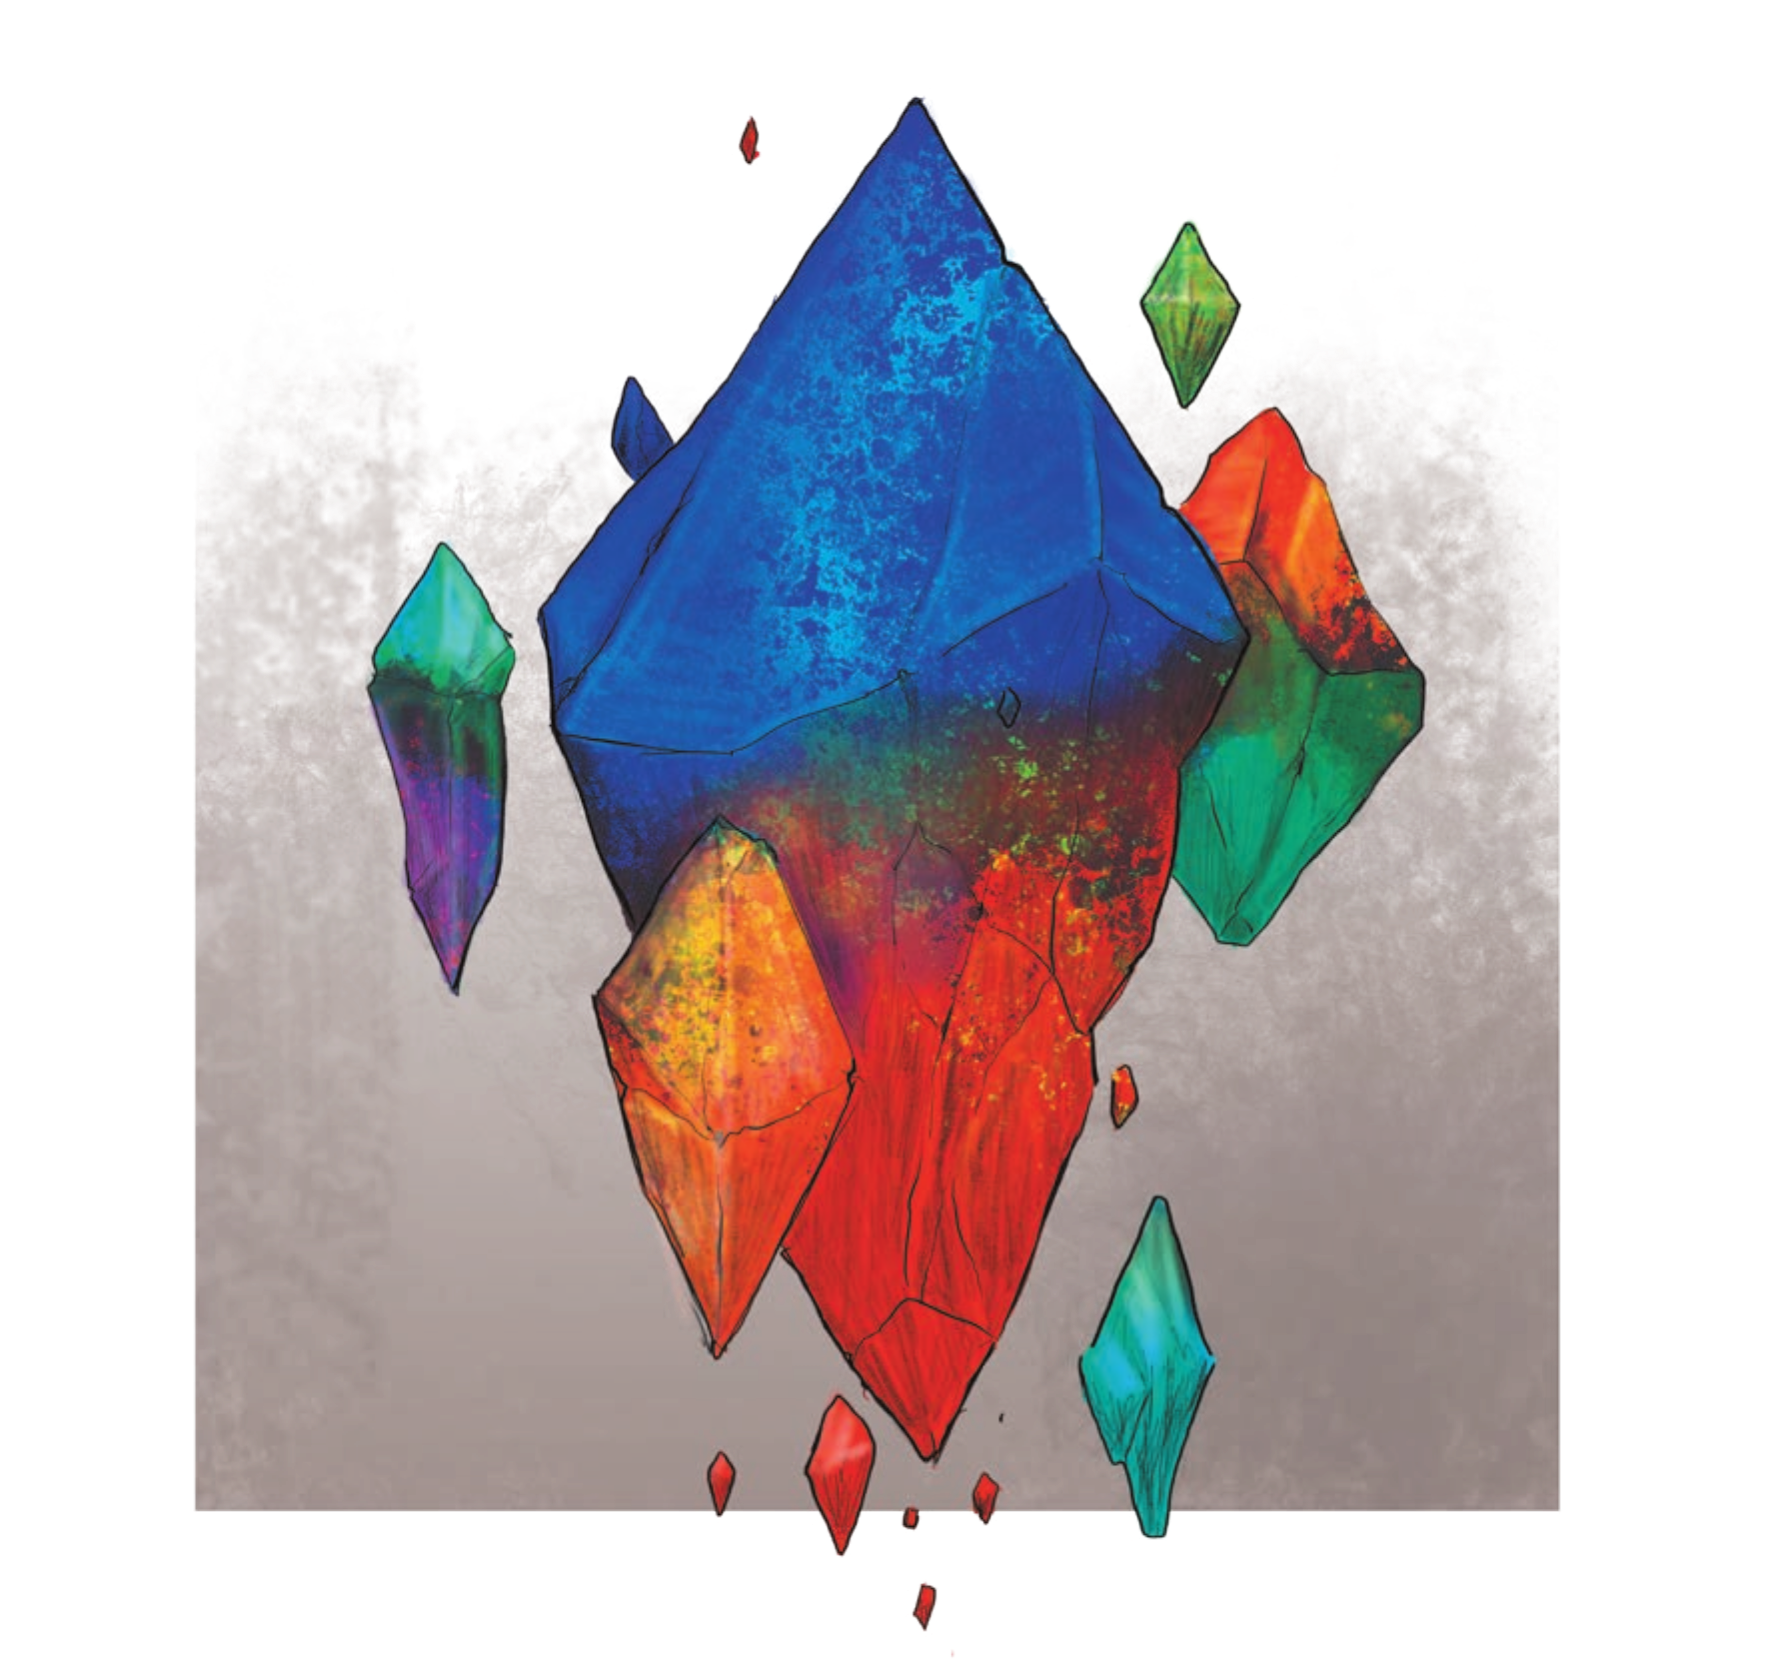
\includegraphics[width=9cm]{images/psionic_crystal.png}
    \caption{Psionic Crystal}
\end{figure}

\section{Manifestations}
Psionic charges are used to manifest psionic abilities. These manifestations are the primary source of a gemstone dragon’s power. All \textbf{manifestations} have a range of 30 feet, unless noted otherwise.\\
The following manifestations are by no means the only ones the dragons have access to. It is known that the most powerful gemstone dragons can alter their form at will in a manner that defies all inspection. But these are the most well-documented and commonly used manifestations available to all psionic creatures.\\
The save DC against a dragon’s manifestation is 8 plus the dragon’s proficiency bonus plus the dragon’s Intelligence modifier.

\DndPsiHeader
  {Amplify}
  {}
  {1 action}
  {Self}
  {4}
  {1 minute}
The dragon focuses the power of its mind and wreaths its teeth, claws, and tail in glowing psionic force. For the next minute, all of its melee attacks deal an extra 3d8 psychic damage.

\DndPsiHeader
  {Distance}
  {}
  {1 action}
  {30 feet}
  {1 per target}
  {Instantaneous}
  Space contorts and twists. Choose any number of targets the dragon can see within 30 feet. Each target must succeed on an Intelligence saving throw or be pushed back 30 feet.

\DndPsiHeader
  {Elsewhere}
  {}
  {1 action}
  {30 feet}
  {2 per 5 feet}
  {Instantaneous}
  Pick a target within 30 feet. The target must succeed on an Intelligence saving throw or be teleported 5 feet per 2 charges spent. The destination must be within sight of the dragon and not currently occupied.

\DndPsiHeader
  {Flay}
  {}
  {1 bonus action}
  {Self (60-foot cone)}
  {2 per d6 of damage}
  {1 round}
  As a bonus action, the dragon blasts pure psionic energy from its eyes, frying the brains of all creatures in a 60-foot cone. Each creature in that area must make an Intelligence saving throw. On a failed save, it takes psychic damage of a d6 per 2 charges spent, or half as much damage on a successful one.

\DndPsiHeader
  {Forget}
  {}
  {1 action}
  {60 feet}
  {5 + 1 per spell level if a spell is chosen}
  {Special}
  The dragon reaches into an enemy’s mind and plucks a critical memory from their cortex, either the knowledge of a spell or of a weapon. This effect lasts until the target finishes a long rest. The dragon can only use this manifestation once per 10 minutes on the same target. Saving against the manifestation means the target is immune to forget for 24 hours.\\
  \textit{Spells:} Pick a target and choose a spell the target knows. Spend charges equal in number to 5 plus the spell level. The target must make a Wisdom saving throw. On a failed save, the target cannot cast that spell until the effect of this manifestation ends.\\
  \textit{Weapons:} Pick a target and choose a weapon. Spend 3 extra charges. The target must make a Wisdom saving throw. On a failed save, the target does not gain the benefit of their proficiency bonus with the chosen kind of weapon while the effect lasts. (For example, they might forget how to use a longsword, but still gain their proficiency benefit with shortswords.)

\DndPsiHeader
  {Mindscape}
  {}
  {1 action}
  {30 feet}
  {3 + 1 per round}
  {Concentration, up to 1 minute}
  The dragon implants a vision of a new landscape in the target’s mind, making them blind to their actual surroundings, causing them to move randomly and erratically. Choose a target to make an Intelligence saving throw. On a failed save, this manifestation becomes active. If the target chooses to move while the manifestation is active, it moves 10 feet in a random direction (roll 1d8) instead of the distance and direction it intended.

\begin{DndComment}{Psionic Magic}
  Although Gemstone Dragons developed separately from the extraplanar marauders, who wield psionics to stun their pray, their psionic manifestations work in a similar way.
  As they are ancient, they are also very aware of those creature.
  They know their tricks and unlike normal magic they can see through them.
\end{DndComment}

\DndPsiHeader
  {Psionic Spell}
  {}
  {determined by the spell}
  {determined by the spell}
  {5 + spell level}
  {determined by the spell}
  The gemstone dragon amplifies a magical spell with its psionic energy.\\
  Choose a spell you know and have prepared.
  You can either cast the spell by expending the appropriate spell slot or as a psionic manifestation.
  If you cast it as a psionic manifestation the spell casting modifier changes to Intelligence and you don't need to expend a spell slot.
  Either way you get the benefit of psionic magic.

\DndPsiHeader
  {Reflection}
  {}
  {1 action }
  {Self}
  {10 + reflection rank}
  {1 minute}
  The dragon reaches through time and plucks an ally from the timescape to come and fight alongside it. Choose a row from the Servitors chart (page 31). The cost of manifesting a reflection is 10 charges plus the type of the summoned creature on the table. (For example, summoning the Inexorable of Nature costs 16 charges: 10 plus the Inexorable’s type of 6.)

\DndPsiHeader
  {Sympathy}
  {}
  {1 reaction}
  {30 feet}
  {2 per d8}
  {Instantaneous}
  The dragon violently reacts to being hurt, raking its enemy’s nervous system with sympathetic psionic vibrations.\\
  As a reaction to taking damage from something the dragon can see within 30 feet, the dragon expends charges to force the damaging creature to make an Intelligence saving throw. On a failed save, the target takes 1d8 psychic damage per 2 charges spent. The maximum damage this can deal equals the damage dealt to the dragon that prompted this manifestation.

\endgroup

% End document
\end{document}
